\documentclass[conference]{IEEEtran}
\IEEEoverridecommandlockouts

\usepackage[utf8]{inputenc}
\usepackage[T1]{fontenc}
\usepackage[brazilian]{babel}
\usepackage{cite}
\usepackage{amsmath,amssymb}
\usepackage{booktabs}
\usepackage{tabularx}
\usepackage{array}
\usepackage{graphicx}
\usepackage{url}
\usepackage[hidelinks]{hyperref}
\usepackage{xspace}

\setlength{\textfloatsep}{6pt plus 1.5pt minus 1.5pt}
\setlength{\dbltextfloatsep}{6pt plus 1.5pt minus 1.5pt}
\setlength{\intextsep}{6pt plus 1.5pt minus 1.5pt}
\setlength{\abovecaptionskip}{3pt}
\setlength{\belowcaptionskip}{1pt}

% Gerado por paper/gera_tabelas.py. Não editar à mão.
\newcommand{\NumMatrizes}{8\xspace}
\newcommand{\NumExecSpmv}{96\xspace}
\newcommand{\NumBitExatas}{96\xspace}
\newcommand{\MinLinhas}{30\xspace}
\newcommand{\MaxLinhas}{1033\xspace}
\newcommand{\MaxNnz}{6027\xspace}
\newcommand{\MedFPtrinta}{$5.91 \times 10^{-8}$\xspace}
\newcommand{\MedTakumTrinta}{$1.15 \times 10^{-8}$\xspace}
\newcommand{\MedFPtrintaAcSes}{$3.61 \times 10^{-8}$\xspace}
\newcommand{\MedTakumTrintaAcTrinta}{$2.94 \times 10^{-8}$\xspace}
\newcommand{\MedTakumTrintaScaled}{$5.37 \times 10^{-9}$\xspace}
\newcommand{\MedBF}{$2.36 \times 10^{-3}$\xspace}
\newcommand{\MedTakumDez}{$7.43 \times 10^{-4}$\xspace}
\newcommand{\MedTakumDezScaled}{$3.09 \times 10^{-4}$\xspace}
\newcommand{\MedTakumOito}{$1.52 \times 10^{-1}$\xspace}
\newcommand{\MedTakumOitoScaled}{$8.39 \times 10^{-2}$\xspace}
\newcommand{\RazaoFormatoAcTrinta}{2.01\xspace}
\newcommand{\RazaoAcumuladorTakum}{2.56\xspace}
\newcommand{\RazaoKernelTrinta}{5.15\xspace}
\newcommand{\RazaoAcAmpliadoTrinta}{3.15\xspace}
\newcommand{\RazaoTakumBF}{3.17\xspace}
\newcommand{\RazaoTakumBFScaled}{7.61\xspace}
\newcommand{\ParTrintaFPAmbos}{8\xspace}
\newcommand{\ParTrintaFPTakumVence}{7\xspace}
\newcommand{\ParTrintaFPOutroVence}{1\xspace}
\newcommand{\ParTrintaFPEmpates}{0\xspace}
\newcommand{\ParTrintaFPTakumNF}{0\xspace}
\newcommand{\ParTrintaFPOutroNF}{0\xspace}
\newcommand{\ParTrintaAcFPAmbos}{8\xspace}
\newcommand{\ParTrintaAcFPTakumVence}{7\xspace}
\newcommand{\ParTrintaAcFPOutroVence}{1\xspace}
\newcommand{\ParTrintaAcFPEmpates}{0\xspace}
\newcommand{\ParTrintaAcFPTakumNF}{0\xspace}
\newcommand{\ParTrintaAcFPOutroNF}{0\xspace}
\newcommand{\ParDezFPAmbos}{5\xspace}
\newcommand{\ParDezFPTakumVence}{3\xspace}
\newcommand{\ParDezFPOutroVence}{2\xspace}
\newcommand{\ParDezFPEmpates}{0\xspace}
\newcommand{\ParDezFPTakumNF}{0\xspace}
\newcommand{\ParDezFPOutroNF}{3\xspace}
\newcommand{\ParDezBFAmbos}{8\xspace}
\newcommand{\ParDezBFTakumVence}{7\xspace}
\newcommand{\ParDezBFOutroVence}{1\xspace}
\newcommand{\ParDezBFEmpates}{0\xspace}
\newcommand{\ParDezBFTakumNF}{0\xspace}
\newcommand{\ParDezBFOutroNF}{0\xspace}
\newcommand{\ParOitoEquatromAmbos}{4\xspace}
\newcommand{\ParOitoEquatromTakumVence}{0\xspace}
\newcommand{\ParOitoEquatromOutroVence}{4\xspace}
\newcommand{\ParOitoEquatromEmpates}{0\xspace}
\newcommand{\ParOitoEquatromTakumNF}{0\xspace}
\newcommand{\ParOitoEquatromOutroNF}{4\xspace}
\newcommand{\ParOitoCincodoisAmbos}{5\xspace}
\newcommand{\ParOitoCincodoisTakumVence}{3\xspace}
\newcommand{\ParOitoCincodoisOutroVence}{2\xspace}
\newcommand{\ParOitoCincodoisEmpates}{0\xspace}
\newcommand{\ParOitoCincodoisTakumNF}{0\xspace}
\newcommand{\ParOitoCincodoisOutroNF}{3\xspace}
\newcommand{\NFTakumOito}{0\xspace}
\newcommand{\NFTakumDez}{0\xspace}
\newcommand{\NFEquatrom}{4\xspace}
\newcommand{\NFCincodois}{3\xspace}
\newcommand{\NFDez}{3\xspace}
\newcommand{\NFBF}{0\xspace}
\newcommand{\ElemNnzFP}{5.33\xspace}
\newcommand{\ElemNnzTakum}{4.50\xspace}
\newcommand{\InsnNnzFPCento}{6.14\xspace}
\newcommand{\CsrNnzFPCento}{1.33\xspace}
\newcommand{\InsnNnzFPDuzentos}{4.59\xspace}
\newcommand{\CsrNnzFPDuzentos}{1.07\xspace}
\newcommand{\InsnNnzFPQuinhentos}{4.34\xspace}
\newcommand{\CsrNnzFPQuinhentos}{1.03\xspace}
\newcommand{\InsnNnzTrintaCento}{5.98\xspace}
\newcommand{\CsrNnzTrintaCento}{1.33\xspace}
\newcommand{\RelInsnTrintaCento}{$-$2.7\%\xspace}
\newcommand{\RelCsrTrintaCento}{+0.0\%\xspace}
\newcommand{\EconomiaCento}{2.7\%\xspace}
\newcommand{\ZvtNnzTrintaCento}{0.50\xspace}
\newcommand{\InsnNnzTrintaDuzentos}{4.55\xspace}
\newcommand{\CsrNnzTrintaDuzentos}{1.07\xspace}
\newcommand{\RelInsnTrintaDuzentos}{$-$0.7\%\xspace}
\newcommand{\RelCsrTrintaDuzentos}{+0.0\%\xspace}
\newcommand{\EconomiaDuzentos}{0.7\%\xspace}
\newcommand{\ZvtNnzTrintaDuzentos}{0.37\xspace}
\newcommand{\InsnNnzTrintaQuinhentos}{4.33\xspace}
\newcommand{\CsrNnzTrintaQuinhentos}{1.03\xspace}
\newcommand{\RelInsnTrintaQuinhentos}{$-$0.3\%\xspace}
\newcommand{\RelCsrTrintaQuinhentos}{+0.0\%\xspace}
\newcommand{\EconomiaQuinhentos}{0.3\%\xspace}
\newcommand{\ZvtNnzTrintaQuinhentos}{0.35\xspace}
\newcommand{\InsnNnzDezCento}{4.95\xspace}
\newcommand{\CsrNnzDezCento}{1.47\xspace}
\newcommand{\RelInsnDezCento}{$-$19.3\%\xspace}
\newcommand{\RelCsrDezCento}{+10.7\%\xspace}
\newcommand{\ZvtNnzDezCento}{0.37\xspace}
\newcommand{\InsnNnzDezDuzentos}{4.69\xspace}
\newcommand{\CsrNnzDezDuzentos}{1.39\xspace}
\newcommand{\RelInsnDezDuzentos}{+2.2\%\xspace}
\newcommand{\RelCsrDezDuzentos}{+29.9\%\xspace}
\newcommand{\ZvtNnzDezDuzentos}{0.35\xspace}
\newcommand{\InsnNnzDezQuinhentos}{4.60\xspace}
\newcommand{\CsrNnzDezQuinhentos}{1.36\xspace}
\newcommand{\RelInsnDezQuinhentos}{+6.0\%\xspace}
\newcommand{\RelCsrDezQuinhentos}{+32.5\%\xspace}
\newcommand{\ZvtNnzDezQuinhentos}{0.34\xspace}
\newcommand{\InsnNnzOitoCento}{4.51\xspace}
\newcommand{\CsrNnzOitoCento}{1.39\xspace}
\newcommand{\RelInsnOitoCento}{$-$26.6\%\xspace}
\newcommand{\RelCsrOitoCento}{+4.6\%\xspace}
\newcommand{\ZvtNnzOitoCento}{0.35\xspace}
\newcommand{\InsnNnzOitoDuzentos}{4.43\xspace}
\newcommand{\CsrNnzOitoDuzentos}{1.36\xspace}
\newcommand{\RelInsnOitoDuzentos}{$-$3.4\%\xspace}
\newcommand{\RelCsrOitoDuzentos}{+27.4\%\xspace}
\newcommand{\ZvtNnzOitoDuzentos}{0.34\xspace}
\newcommand{\InsnNnzOitoQuinhentos}{4.39\xspace}
\newcommand{\CsrNnzOitoQuinhentos}{1.35\xspace}
\newcommand{\RelInsnOitoQuinhentos}{+1.1\%\xspace}
\newcommand{\RelCsrOitoQuinhentos}{+31.2\%\xspace}
\newcommand{\ZvtNnzOitoQuinhentos}{0.34\xspace}
\newcommand{\InsnMenorTrinta}{13\xspace}
\newcommand{\InsnIgualTrinta}{11\xspace}
\newcommand{\InsnMaiorTrinta}{0\xspace}
\newcommand{\InsnMenorDez}{11\xspace}
\newcommand{\InsnIgualDez}{0\xspace}
\newcommand{\InsnMaiorDez}{13\xspace}
\newcommand{\InsnMenorOito}{12\xspace}
\newcommand{\InsnIgualOito}{0\xspace}
\newcommand{\InsnMaiorOito}{12\xspace}
\newcommand{\InsnPares}{24\xspace}
\newcommand{\ModRFP}{13\xspace}
\newcommand{\ModCFP}{12\xspace}
\newcommand{\ModKFP}{21\xspace}
\newcommand{\ModROito}{14\xspace}
\newcommand{\ModCOito}{12\xspace}
\newcommand{\ModKOito}{21\xspace}
\newcommand{\ModRDez}{14\xspace}
\newcommand{\ModCDez}{13\xspace}
\newcommand{\ModKDez}{21\xspace}
\newcommand{\ModRTrinta}{14\xspace}
\newcommand{\ModCTrinta}{11\xspace}
\newcommand{\ModKTrinta}{21\xspace}
\newcommand{\ModExatas}{96\xspace}
\newcommand{\ModExec}{96\xspace}
\newcommand{\ModSinteticosOk}{12\xspace}
\newcommand{\ModSinteticosTotal}{12\xspace}
\newcommand{\ModResiduoMax}{0\xspace}


\author{\IEEEauthorblockN{Andr\'e Lu\'is Alves Rezende, Gabriel Ramos Fontes,
Isadora Maria Carvalho Lopes, Jo\~ao Pedro Santos de Brito}
\IEEEauthorblockA{Departamento de Engenharia Eletr\^onica (DELT), Universidade Federal de Minas Gerais (UFMG)\\
Belo Horizonte, MG, Brasil}}

\title{Implementa\c{c}\~ao e Avalia\c{c}\~ao do Formato Aritm\'etico Takum na Extens\~ao Vetorial RISC-V (Zvtakum)}

\begin{document}
\renewcommand{\abstractname}{Resumo}
\renewcommand{\IEEEkeywordsname}{Palavras-chave}
\renewcommand{\refname}{Refer\^encias}
\renewcommand{\figurename}{Fig.}
\renewcommand{\tablename}{TABELA}
\maketitle

\begin{abstract}
Variantes de ponto flutuante de baixa precis\~ao (IEEE FP16, bfloat16, OCP FP8 E4M3/E5M2) inflam conjuntos de instru\c{c}\~oes vetoriais com decodificadores fragmentados, caminhos de subnormais, convers\~oes cruzadas e riscos em registradores de controle/estado. A aritm\'etica Takum oferece precis\~ao afilada (\emph{tapered precision}), faixa din\^amica limitada e janela unificada de decodifica\c{c}\~ao nos 12 bits mais significativos (MSBs) para qualquer largura. Apresentamos a \texttt{Zvtakum}, extens\~ao experimental para a Extens\~ao Vetorial RISC-V (RVV~1.0) com suporte a \texttt{T8}, \texttt{T16} e \texttt{T32} via cinco instru\c{c}\~oes em \texttt{custom-0}: \texttt{vtadd.vv}, \texttt{vtsub.vv}, \texttt{vtmul.vv}, \texttt{vtdot.vv} (acumula\c{c}\~ao em largura dupla) e \texttt{vncvt.t.t} (estreitamento). Projetamos uma ULA Takum em inteiros de 128 bits com arredondamento ao par mais pr\'oximo no espa\c{c}o de c\'odigos (RNE) integrada a um simulador funcional RV64IM, Zicsr, RVV~1.0 e \texttt{Zvtakum}. A verifica\c{c}\~ao abrange tabelas exaustivas \texttt{T8} contra a \texttt{libtakum}, or\'aculo \texttt{binary128} contra \texttt{libquadmath}, testes diferenciais contra o QEMU~10.2.2 para $\mathrm{VLEN}\in\{128,256,512\}$ e \NumExecSpmv\ execu\c{c}\~oes bit a bit exatas de multiplica\c{c}\~ao matriz esparsa--vetor (SpMV) em oito matrizes Harwell--Boeing. Em acumuladores iguais de 32 bits, \texttt{Takum32} reduz o erro relativo $\ell_2$ mediano em $\RazaoFormatoAcTrinta\times$ frente ao \texttt{FP32} (e $\RazaoKernelTrinta\times$ com acumula\c{c}\~ao \texttt{T64}). Ao contr\'ario de \texttt{E4M3}, \texttt{E5M2} e \texttt{FP16} sem reescalamento---que sofrem \emph{overflows} n\~ao finitos em 3--4 de 8 matrizes---, \texttt{Takum8} e \texttt{Takum16} permanecem 100\% finitos e \texttt{Takum16} supera \texttt{bfloat16} em 7/8 execu\c{c}\~oes n\~ao escaladas e 8/8 escaladas. Um modelo anal\'itico exato ($N_f = r_f R + c_f S + K$) reproduz todas as execu\c{c}\~oes com res\'iduo nulo e prova que \texttt{Takum32} nunca ultrapassa a contagem de instru\c{c}\~oes do \texttt{FP32}.
\end{abstract}

\begin{IEEEkeywords}
RISC-V, RVV, aritm\'etica Takum, precis\~ao afilada, Zvtakum, SpMV, simulador funcional.
\end{IEEEkeywords}

\section{Introdu\c{c}\~ao}
Processadores vetoriais e SIMD modernos voltados \`a intelig\^encia artificial e computa\c{c}\~ao cient\'ifica esparsa s\~ao limitados principalmente pela largura de banda de mem\'oria. Para compactar mais operandos por registrador vetorial, arquiteturas adotaram m\'ultiplas variantes IEEE~754 de baixa precis\~ao, como meia precis\~ao (\texttt{FP16}), \texttt{bfloat16}~\cite{bfloat16} e os formatos de 8 bits do \emph{Open Compute Project} (\texttt{OFP8 E4M3} e \texttt{E5M2})~\cite{ofp8,micikevicius2022fp8}. Contudo, particionamentos bin\'arios fixos imp\~oem um compromisso r\'igido entre faixa din\^amica e mantissa, gerando subformatos incompat\'iveis, casos de exce\c{c}\~ao, deslocadores de subnormais, m\'ultiplos NaNs e $O(N^2)$ instru\c{c}\~oes de convers\~ao cruzada~\cite{hunhold2025avx102}. Na extens\~ao vetorial RISC-V (RVV~1.0)~\cite{riscv-v-spec}, \texttt{FP8} sequer existe, \texttt{FP16} depende da \texttt{Zvfh} e \texttt{bfloat16} acrescenta extens\~oes pr\'oprias de convers\~ao (\texttt{Zvfbfmin}/\texttt{Zvfbfwma}).

A aritm\'etica Takum~\cite{hunhold2024takum} supera esses gargalos de hardware e ISA ao combinar precis\~ao afilada com um prefixo n\~ao fracion\'ario limitado aos 12 MSBs em qualquer largura de palavra. Inspirados pelo estudo de enxugamento do Intel AVX10.2 por Hunhold~\cite{hunhold2025avx102}, especificamos, implementamos e avaliamos a extens\~ao \texttt{Zvtakum} sobre RVV~1.0. Nossas contribui\c{c}\~oes s\~ao:
\begin{enumerate}
    \item Codec e ULA Takum em inteiros de 128 bits para \texttt{T8}/\texttt{T16}/\texttt{T32} (acumula\c{c}\~ao \texttt{T64}) implementando a sem\^antica linear da Defini\c{c}\~ao~8 e RNE no espa\c{c}o de c\'odigos sem ponto flutuante do hospedeiro;
    \item A ISA \texttt{Zvtakum} com cinco instru\c{c}\~oes em \texttt{custom-0} integradas a um \emph{datapath} RISC-V/RVV sem riscos em \texttt{fcsr};
    \item Verifica\c{c}\~ao diferencial frente ao QEMU~10.2.2~\cite{qemu}, \texttt{libtakum}~\cite{libtakum}, \texttt{libquadmath} e or\'aculo racional exato em Python;
    \item Avalia\c{c}\~oes de precis\~ao e contagem de instru\c{c}\~oes em SpMV ($y = A\cdot x$) e 100 matrizes SuiteSparse frente a \texttt{FP32/FP16}, \texttt{bfloat16}, \texttt{OFP8} (padr\~ao e saturante), reescalamento \texttt{pow2-bound}, \texttt{Posit} e Takum logar\'itmico.
\end{enumerate}

\section{Fundamenta\c{c}\~ao Te\'orica e Trabalhos Relacionados}

\subsection{Derivados IEEE de Baixa Precis\~ao e Aritm\'etica Posit}
Formatos bin\'arios IEEE~754~\cite{ieee754} dividem bits rigidamente entre sinal, expoente e fra\c{c}\~ao. O \texttt{FP16} (10 bits de fra\c{c}\~ao) oferece boa precis\~ao local pr\'oxima a~1, por\'em sua faixa estreita ($\approx 10^{\pm 5}$) transborda sem reescalamento. O \texttt{bfloat16}~\cite{bfloat16} preserva o expoente de 8 bits do \texttt{FP32} ($\approx 10^{\pm 38}$) com apenas 7 bits fracion\'arios, enquanto o \texttt{OFP8} se divide em \texttt{E4M3} ($[-448,448]$) e \texttt{E5M2} ($[-57344,57344]$)~\cite{ofp8}. A aritm\'etica Posit~\cite{gustafson2017posit} introduziu precis\~ao afilada com apenas $0$ e \texttt{NaR}, mas seu regime un\'ario exige detectores de zeros/uns \`a esquerda em toda a palavra e o \texttt{Posit8} ($es=2$) cobre somente $[2^{-24}, 2^{24}]$.

\begin{figure*}[t]
\centering
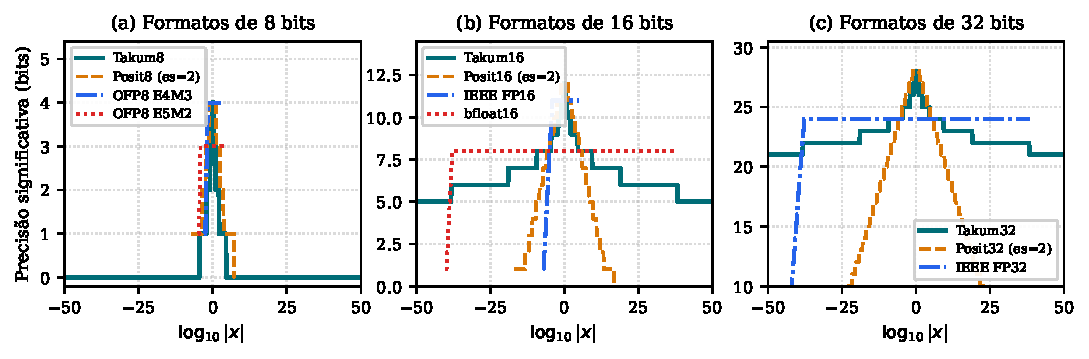
\includegraphics[width=0.77\textwidth]{figures/tapered-precision-pt.pdf}
\caption{Precis\~ao significativa ($1+p$ bits) em fun\c{c}\~ao da escala ($\log_{10}|x|$) nos formatos de 8, 16 e 32 bits. O formato Takum mant\'em precis\~ao afilada perto da unidade cobrindo $\approx 10^{\pm 72}$ (\texttt{T8}) a $10^{\pm 77}$ (\texttt{T16/T32}) via cabe\c{c}alho fixo de 12~MSBs, evitando o colapso de precis\~ao dos posits nos extremos.}
\label{fig:tapered}
\end{figure*}

\subsection{Codifica\c{c}\~ao Takum e Janela Unificada de 12 MSBs}
Uma palavra Takum de $n$ bits $X[n-1:0]$ concatena, do MSB ao LSB, sinal $S$ (1 bit), dire\c{c}\~ao $D$ (1 bit), regime $R$ (3 bits), caracter\'istica vari\'avel $C$ ($r$ bits) e fra\c{c}\~ao $F$ ($p = n - 5 - r$ bits)~\cite{hunhold2024takum}. Os padr\~oes reservados s\~ao $0\dots0$ (zero) e $10\dots0$ (\texttt{NaR}), sem zero sinalizado nem infinito; a nega\c{c}\~ao por complemento de dois preserva ordena\c{c}\~ao total. A largura $r \in \{0,\dots,7\}$ decorre diretamente de $D$ e $R$:
\begin{equation}
    r = \begin{cases} 7 - \mathrm{uint}(R), & D = 0 \\ \mathrm{uint}(R), & D = 1 \end{cases},\quad
    L_{\max} = 5 + 7 = 12~\text{bits}.
\end{equation}
Como $r \le 7$, o prefixo de escala $(S, D, R, C)$ cabe nos 12~MSBs em qualquer largura. Para $n < 12$ (\texttt{T8}), desloca-se a palavra $12 - n = 4$ bits \`a esquerda preenchendo \emph{ghost bits} nulos \`a direita~\cite{hunhold2024takum}, restringindo o expoente de \texttt{T8} a $[-239, +239]$ ($\approx 10^{\pm 72}$) com a mesma l\'ogica decodificadora de \texttt{T16} e \texttt{T32}.

Na variante \emph{Takum linear} (Defini\c{c}\~ao~8 de~\cite{hunhold2024takum}) adotada para ULAs vetoriais, a caracter\'istica sinalizada $c$ e o valor exato $v$ s\~ao:
\begin{equation}
    c = \begin{cases} -(2^{r+1}-1) + \mathrm{uint}(C), & D = 0 \\ (2^r - 1) + \mathrm{uint}(C), & D = 1 \end{cases}
\end{equation}
\begin{equation}
    v = (-1)^S \left(1 - 3S + \frac{\mathrm{uint}(F)}{2^p}\right) \cdot 2^{(-1)^S (c + S)},
\end{equation}
decompondo-se no significando inteiro $N = 2^p + F$ ($S=0$) ou $N = 2^{p+1} - F$ ($S=1$) escalado por $2^{c-p}$ ou $2^{-(c+1)-p}$. A Fig.~\ref{fig:tapered} mostra maior precis\~ao junto \`a unidade que \texttt{FP16}, \texttt{bfloat16} e \texttt{FP32} ($12$ bits em \texttt{T16}, $28$ bits em \texttt{T32}) e piso de resolu\c{c}\~ao garantido nas caudas ($5$ e $21$ bits) em $\approx 10^{\pm 77}$. J\'a o \emph{Takum logar\'itmico} (Defini\c{c}\~ao~2 de~\cite{hunhold2024takum}, $v = (-1)^S \sqrt{e}^{\ell}$) transforma multiplica\c{c}\~ao e invers\~ao em somas inteiras---atingindo 41.2\% (\texttt{T8}) e 36.7\% (\texttt{T16}) de fechamento multiplicativo contra 33.7\% e 1.2\% no Takum linear---, por\'em sua soma exige tabelas n\~ao lineares $\Delta_\pm$, ao passo que o Takum linear mant\'em ULAs inteiras compat\'iveis com RVV~\cite{hunhold2025avx102}.

\subsection{Trabalhos Relacionados}
Hunhold~\cite{hunhold2025avx102} mostrou que substituir variantes SIMD do AVX10.2 por Takum reduz tabelas de instru\c{c}\~oes e melhora a acur\'acia em 1.401 matrizes SuiteSparse~\cite{davis2011suitesparse,mufolab}, e implementou um codec VHDL com at\'e 38\% menor lat\^encia e 50\% menos LUTs que posits~\cite{hunhold2024vhdl}. Estudos em resolvedores esparsos~\cite{hunhold2025solvers}, m\'etodo de Arnoldi~\cite{hunhold2025arnoldi} e exatid\~ao inteira~\cite{hunhold2025integers} comprovam estabilidade frente a \texttt{bfloat16} e \texttt{OFP8}. No ecossistema RISC-V, PERCIVAL~\cite{mallasen2022percival} e Cococcioni et al.~\cite{cococcioni2021vectorizing} exploraram posits com \emph{quire}; FPnew~\cite{mach2020fpnew} e FAUST~\cite{kovac2023faust} constru\'iram FPUs vetoriais multiformato; e Marcelli et al.~\cite{marcelli2025fp8spike} adicionaram FP8 SoftFloat ao Spike. Diferentemente desses trabalhos, \texttt{Zvtakum} entrega aritm\'etica vetorial Takum unificada sobre RVV~1.0 com ULA inteira de 128 bits e valida\c{c}\~ao diferencial por instru\c{c}\~ao.

\section{Metodologia e Arquitetura Proposta}

\subsection{Reestrutura\c{c}\~ao da RVV e Codifica\c{c}\~ao \texttt{Zvtakum}}
Um levantamento no \texttt{riscv-opcodes}~\cite{riscv-opcodes} contabiliza 510 instru\c{c}\~oes vetoriais (RVV~1.0, \texttt{bfloat16} \texttt{Zvfbfmin}/\texttt{Zvfbfwma} e criptografia \texttt{Zvk*}), sendo 92 de ponto flutuante e 4 de \texttt{bfloat16} (25 convers\~oes). Pela metodologia do AVX10.2~\cite{hunhold2025avx102}, parametrizar \texttt{T8}/\texttt{T16}/\texttt{T32} via \texttt{vtype.vsew} reduz essas 96 opera\c{c}\~oes a oito primitivas Takum (\texttt{vtadd}, \texttt{vtsub}, \texttt{vtmul}, \texttt{vtdiv}, \texttt{vtsqrt}, \texttt{vtdot}, \texttt{vncvt.t.t} e convers\~oes inteiras), reaproveitando compara\c{c}\~oes inteiras em complemento de dois~\cite{hunhold2024takum}.

\begin{table}[t]
\caption{Instru\c{c}\~oes \texttt{Zvtakum} Propostas em \texttt{custom-0} (\texttt{0x0B}, \texttt{funct3=000}).}
\label{tab:zvtakum_isa}
\centering
\scriptsize
\setlength{\tabcolsep}{3.0pt}
\begin{tabular}{@{}llll@{}}
\toprule
\textbf{Mnem\^onico} & \textbf{funct6} & \textbf{Equiv. RVV} & \textbf{Sem\^antica Operacional} \\
\midrule
\texttt{vtadd.vv} & \texttt{000000} & \texttt{vfadd.vv} & $vd[i] = vs2[i] + vs1[i]$ (\texttt{SEW}) \\
\texttt{vtsub.vv} & \texttt{000001} & \texttt{vfsub.vv} & $vd[i] = vs2[i] - vs1[i]$ (\texttt{SEW}) \\
\texttt{vtmul.vv} & \texttt{000010} & \texttt{vfmul.vv} & $vd[i] = vs2[i] \times vs1[i]$ (\texttt{SEW}) \\
\texttt{vtdot.vv} & \texttt{000011} & \texttt{vfdot.vv} & $vd[0]_{2\mathrm{SEW}} \mathrel{+}= \sum_i vs2[i]\cdot vs1[i]$ \\
\texttt{vncvt.t.t} & \texttt{000100} & \texttt{vfncvt.*} & $vd[i]_{\mathrm{SEW}} = \mathrm{narrow}(vs2[i]_{2\mathrm{SEW}})$ \\
\bottomrule
\end{tabular}
\vspace{2pt}
\raggedright\footnotesize{Codifica\c{c}\~ao em \texttt{custom-0} (\texttt{funct6}=0..4); bit~25 (\texttt{vm}) seleciona m\'ascara \texttt{v0}; \texttt{vncvt.t.t} exige \texttt{vs1=00000}.}
\end{table}

A Tabela~\ref{tab:zvtakum_isa} lista as cinco instru\c{c}\~oes implementadas. Em vez de sobrecarregar \texttt{OP-V} assumindo um \texttt{funct6} livre \'unico, alocamos \texttt{Zvtakum} em \texttt{custom-0} (\texttt{opcode=0x0B}, \texttt{funct3=000}, \texttt{funct6=0..4}), preservando \texttt{OP-V}. As opera\c{c}\~oes elemento a elemento suportam $\mathrm{SEW}\in\{8,16,32\}$ e $\mathrm{LMUL}\in\{1,2,4,8\}$, obedecendo a \texttt{vl}, \texttt{vstart}, m\'ascara \texttt{v0.t} e pol\'iticas \texttt{vta}/\texttt{vma}. A instru\c{c}\~ao \texttt{vtdot.vv} acumula produtos ativos sequencialmente em \texttt{vd[0]} com $\mathrm{EEW}=2\cdot\mathrm{SEW}$ ($\mathrm{EMUL}=1$, habilitando acumula\c{c}\~ao interna \texttt{T64} para operandos \texttt{T32} sem expor vetores \texttt{T64}), enquanto \texttt{vncvt.t.t} estreita um grupo alinhado $2\cdot\mathrm{LMUL}$ para \texttt{SEW}.

\subsection{Integra\c{c}\~ao no Caminho de Dados RISC-V + \texttt{Zvtakum}}
\begin{figure*}[t]
\centering
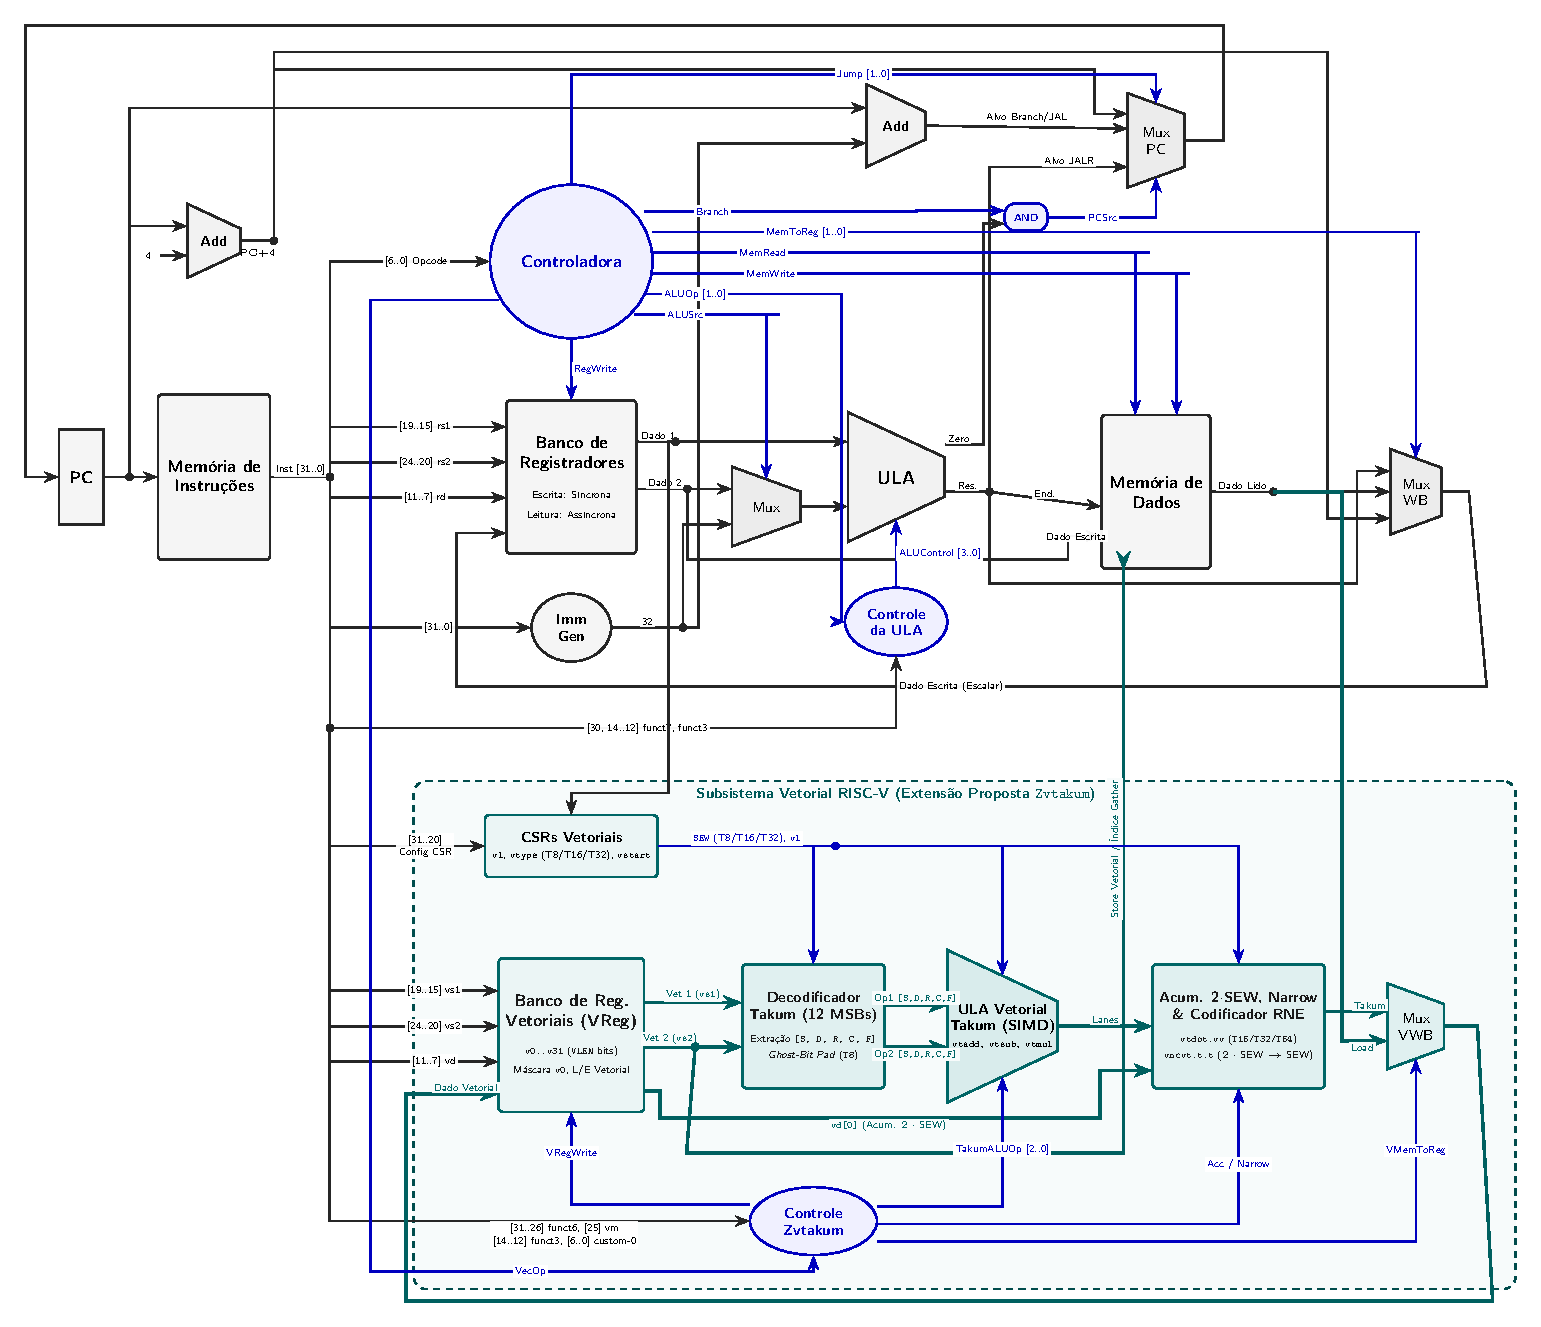
\includegraphics[width=0.61\textwidth]{figures/datapath_zvtakum_pt.pdf}
\caption{Caminho de dados RISC-V proposto com subsistema vetorial \texttt{Zvtakum} (em azul-petr\'oleo). Um \'unico decodificador de 12~MSBs alimenta as vias SIMD da ULA Takum, o acumulador/estreitador $2\cdot\text{SEW}$ e o \texttt{MuxVWB}, reutilizando o c\'alculo escalar de endere\c{c}os para cargas/armazenamentos e \emph{gathers} indexados.}
\label{fig:datapath}
\end{figure*}

A Fig.~\ref{fig:datapath} ilustra a integra\c{c}\~ao sobre o n\'ucleo RISC-V:
\begin{itemize}
    \item \textbf{CSRs (\texttt{vl}, \texttt{vtype}, \texttt{vstart}) e \texttt{VReg}:} Atualizados via \texttt{vsetvl*} por \texttt{rs1}; \texttt{VReg} prov\^e 32 registradores de $\mathrm{VLEN}$ bits (\texttt{vs1}/\texttt{vs2}/\texttt{vd}).
    \item \textbf{Decodificador Unificado de 12 MSBs:} Extrai $[S,D,R,C,F]$ de forma id\^entica para \texttt{T8}, \texttt{T16} e \texttt{T32} (com \emph{ghost bits} em \texttt{T8}).
    \item \textbf{ULA Vetorial \& Acumulador $2\cdot\text{SEW}$:} Executa \texttt{vtadd}/\texttt{vtsub}/\texttt{vtmul}, acumula \texttt{vd[0]} em $2\cdot\text{SEW}$ em \texttt{vtdot.vv}, estreita $2\cdot\text{SEW}\to\text{SEW}$ em \texttt{vncvt.t.t} e aplica codifica\c{c}\~ao RNE antes do \texttt{MuxVWB}.
    \item \textbf{Elimina\c{c}\~ao de Riscos em \texttt{fcsr}:} RNE determin\'istico, satura\c{c}\~ao em $[\mathrm{minpos}, \mathrm{maxpos}]$ sem infinito e propaga\c{c}\~ao alg\'ebrica de \texttt{NaR} eliminam \texttt{frm} e redu\c{c}\~oes de \texttt{fflags} entre vias SIMD.
\end{itemize}

\subsection{ULA Takum em Inteiros de 128 Bits e RNE no Espa\c{c}o de C\'odigos}
O n\'ucleo C++17 (\texttt{src/takum.cpp}) opera exclusivamente em \texttt{uint64\_t} e \texttt{unsigned \_\_int128}, evitando intermedi\'arios \texttt{double}. A decodifica\c{c}\~ao extrai $(\mathrm{neg}, e, \mathrm{sig})$ para $(-1)^{\mathrm{neg}}\cdot\mathrm{sig}\cdot 2^{e-63}$. A soma alinha os operandos em 128 bits com bit \emph{sticky} (reusado como \emph{borrow} na subtra\c{c}\~ao efetiva); a multiplica\c{c}\~ao produz produto exato de 128 bits e \emph{sticky}. Na codifica\c{c}\~ao positiva, $(D,R,C)$ e a fra\c{c}\~ao de $\mathrm{sig}$ s\~ao empacotados em \texttt{u128}, extraindo prefixo $L$ ($n$ bits), bit m\'edio $m$ e cauda $\mathit{st}$; incrementa-se $L\to L+1$ sse $m=1 \land (\mathit{st} \lor (L\bmod 2 = 1))$, saturando em $[1, 2^{n-1}-1]$ antes do complemento de dois se $\mathrm{neg}=1$. Esse RNE no espa\c{c}o de c\'odigos segue fielmente o hardware~\cite{hunhold2024vhdl}; por exemplo, na fronteira $p=0$ de \texttt{T8}, $2^{-231}$ \'e o ponto geom\'etrico m\'edio entre o c\'odigo~1 ($2^{-239}$) e o c\'odigo~2 ($2^{-223}$), arredondando para o c\'odigo par~2.

\section{Verifica\c{c}\~ao e Metodologia Experimental}

\subsection{Verifica\c{c}\~ao Multicamadas}
Quatro camadas independentes asseguram equival\^encia bit a bit:
\begin{enumerate}
    \item \textbf{Codec/ULA vs.\ Racionais Exatos:} Verifica\c{c}\~ao exaustiva em \texttt{T8} (\texttt{add}, \texttt{sub}, \texttt{mul}; $3\times 65.536$ pares) e \texttt{T16$\to$T8} ($65.536$ estreitamentos), ciclos completos \texttt{T8}/\texttt{T16}, e $24.000+$ vetores \texttt{T16/T32/T64} e \texttt{vtdot} contra modelo Python \texttt{Fraction} (0 falhas em 73 verifica\c{c}\~oes C++ e 18 testes Python).
    \item \textbf{\texttt{libtakum} e Duplo Arredondamento:} Todas as 256 decodifica\c{c}\~oes, 196.608 opera\c{c}\~oes \texttt{T8} e 50.000 testes \texttt{T16} coincidem com a \texttt{libtakum}~v2.0.0~\cite{libtakum} (0 diverg\^encias). Em 30.000 testes \texttt{T32}, 128 produtos pr\'oximos ao empate (ex.: $\texttt{0x40000001} \times \texttt{0x44000001}$) diferem por 1~ULP porque a \texttt{libtakum} usa \texttt{double} em C, enquanto nossa ULA de 128 bits preserva o desempate racional exato.
    \item \textbf{Or\'aculo \texttt{binary128}:} Nosso or\'aculo \texttt{Float128} coincide com o GCC~9.4.0 \texttt{\_\_float128}/\texttt{libquadmath} em 6.017 testes (diferindo apenas em tr\^es normaliza\c{c}\~oes documentadas de zero sinalizado).
    \item \textbf{Simulador vs.\ QEMU~10.2.2:} O \texttt{zt-sim} coincide byte a byte com \texttt{qemu-riscv64} para $\mathrm{VLEN}\in\{128,256,512\}$ em RV64IM/Zicsr e RVV~1.0 (m\'ascaras, caudas, \texttt{vl} parcial, $\mathrm{vl}=0$, \texttt{vstart}, \texttt{LMUL}=2, \texttt{vluxei32}), e com o modelo Python em \texttt{Zvtakum}.
\end{enumerate}

\subsection{Kernels SpMV, Reescalamento e Matrizes SuiteSparse}
Avaliamos a SpMV em CSR ($y = A\cdot x$) sobre oito matrizes Harwell--Boeing~\cite{duff1989hb} (\texttt{bcsstk01}, \texttt{bcsstk02}, \texttt{jpwh\_991}, \texttt{pores\_1}, \texttt{sherman1}, retangular \texttt{well1033}, \texttt{west0067}, \texttt{west0132}; $\MinLinhas$--$\MaxLinhas$ linhas, at\'e $\MaxNnz$ n\~ao nulos) com vetor $x_j = k_j/2^{52}$ ($\text{seed}=2026$). Os kernels \texttt{FP32} e \texttt{Takum} compartilham exatamente a malha escalar e o \emph{gather} (\texttt{vluxei32.v}):
\begin{itemize}
    \item \textbf{Faixa \texttt{FP32}:} \texttt{vsetvli}, \texttt{vle32} (\'indices), \texttt{vle32} (valores), \texttt{vluxei32}, \texttt{vfmul.vv}, \texttt{vfredusum.vs} e ponteiros (12 instr./faixa).
    \item \textbf{Faixa \texttt{Takum$n$}:} \texttt{vsetvli} (com troca de \texttt{EMUL} para $n\in\{8,16\}$), \texttt{vle32}, \texttt{vle$n$}, \texttt{vluxei32}, \texttt{vtdot.vv}, ponteiros e \texttt{vncvt.t.t} uma vez por linha.
\end{itemize}
Para \texttt{OFP8} (\texttt{E4M3}, \texttt{E5M2}, e variantes saturantes \texttt{E4M3\_sat}, \texttt{E5M2\_sat}), \texttt{FP16} e \texttt{bfloat16}, avaliamos refer\^encias num\'ericas racionais exatas com a mesma ordem de redu\c{c}\~ao nos regimes sem reescalamento (\texttt{none}) e com reescalamento por pot\^encia de dois na norma infinito (\texttt{pow2-bound}). Inclu\'imos ainda 100 matrizes SuiteSparse ($\mathrm{nnz}\le 50{.}000$) em 15 formatos para comparar com \texttt{Posit} (\texttt{es=2}) e Takum logar\'itmico.

\section{Resultados e Discuss\~ao}

\begin{table*}[t]
\caption{Erro relativo $\ell_2$ no SpMV em 32 bits (VLEN = 256) frente ao Float128, por matriz. FP32 e Takum32 são kernels RISC-V simulados (acumuladores de 32 e 64 bits); os controles isolam a largura do acumulador e o pré-escalonamento \texttt{pow2-bound}.}
\label{tab:precisao32}
\centering
\footnotesize
\begin{tabular}{@{}lrccccc@{}}
\toprule
Matriz & nnz & FP32 (ac. 32b) & Takum32 (ac. 64b) & FP32 (ac. 64b) & Takum32 (ac. 32b) & Takum32 (esc.) \\
\midrule
bcsstk01 & 400 & $7.20 \times 10^{-8}$ & $5.06 \times 10^{-8}$ & $3.57 \times 10^{-8}$ & $6.22 \times 10^{-8}$ & $3.54 \times 10^{-9}$ \\
bcsstk02 & 4356 & $1.81 \times 10^{-7}$ & $1.88 \times 10^{-8}$ & $4.63 \times 10^{-8}$ & $8.32 \times 10^{-8}$ & $7.40 \times 10^{-9}$ \\
jpwh\_991 & 6027 & $6.32 \times 10^{-8}$ & $4.19 \times 10^{-9}$ & $3.47 \times 10^{-8}$ & $9.40 \times 10^{-9}$ & $4.38 \times 10^{-9}$ \\
pores\_1 & 180 & $3.54 \times 10^{-8}$ & $7.87 \times 10^{-8}$ & $3.26 \times 10^{-8}$ & $5.44 \times 10^{-8}$ & $5.11 \times 10^{-9}$ \\
sherman1 & 3750 & $5.82 \times 10^{-8}$ & $4.02 \times 10^{-9}$ & $3.65 \times 10^{-8}$ & $4.93 \times 10^{-9}$ & $5.62 \times 10^{-9}$ \\
well1033 & 4732 & $5.99 \times 10^{-8}$ & $4.07 \times 10^{-9}$ & $3.72 \times 10^{-8}$ & $6.45 \times 10^{-9}$ & $6.94 \times 10^{-9}$ \\
west0067 & 294 & $4.82 \times 10^{-8}$ & $3.59 \times 10^{-9}$ & $3.27 \times 10^{-8}$ & $4.84 \times 10^{-9}$ & $6.18 \times 10^{-9}$ \\
west0132 & 413 & $5.01 \times 10^{-8}$ & $3.21 \times 10^{-8}$ & $4.00 \times 10^{-8}$ & $4.94 \times 10^{-8}$ & $2.72 \times 10^{-9}$ \\
\midrule
Mediana & & $5.91 \times 10^{-8}$ & $1.15 \times 10^{-8}$ & $3.61 \times 10^{-8}$ & $2.94 \times 10^{-8}$ & $5.37 \times 10^{-9}$ \\
\bottomrule
\end{tabular}
\end{table*}

\begin{table*}[t]
\caption{Erro relativo $\ell_2$ no SpMV em 8 e 16 bits frente ao Float128 (VLEN = 256). NF($k$) indica $k$ linhas não finitas (overflow). Acumuladores: 16 bits para E4M3, E5M2 e Takum8; 32 bits para FP16, bfloat16 e Takum16. O rodapé resume o efeito do escalonamento \texttt{pow2-bound}.}
\label{tab:precisao816}
\centering
\footnotesize
\begin{tabular}{@{}lcccccc@{}}
\toprule
Matriz & E4M3 & E5M2 & FP16 & bfloat16 & Takum16 & Takum8 \\
\midrule
bcsstk01 & NF(48) & NF(48) & NF(48) & $2.28 \times 10^{-3}$ & $3.24 \times 10^{-3}$ & $6.44 \times 10^{-1}$ \\
bcsstk02 & NF(66) & $7.31 \times 10^{-2}$ & $3.76 \times 10^{-4}$ & $2.43 \times 10^{-3}$ & $1.20 \times 10^{-3}$ & $2.27 \times 10^{-1}$ \\
jpwh\_991 & $3.45 \times 10^{-2}$ & $7.58 \times 10^{-2}$ & $2.77 \times 10^{-4}$ & $2.26 \times 10^{-3}$ & $3.04 \times 10^{-4}$ & $7.77 \times 10^{-2}$ \\
pores\_1 & NF(30) & NF(15) & NF(15) & $1.53 \times 10^{-3}$ & $1.18 \times 10^{-3}$ & $8.58 \times 10^{-1}$ \\
sherman1 & $3.95 \times 10^{-2}$ & $1.00 \times 10^{-1}$ & $3.06 \times 10^{-4}$ & $2.68 \times 10^{-3}$ & $2.28 \times 10^{-4}$ & $6.40 \times 10^{-2}$ \\
well1033 & $4.24 \times 10^{-2}$ & $8.75 \times 10^{-2}$ & $3.54 \times 10^{-4}$ & $2.53 \times 10^{-3}$ & $2.62 \times 10^{-4}$ & $6.47 \times 10^{-2}$ \\
west0067 & $3.43 \times 10^{-2}$ & $8.74 \times 10^{-2}$ & $3.36 \times 10^{-4}$ & $2.52 \times 10^{-3}$ & $1.76 \times 10^{-4}$ & $5.18 \times 10^{-2}$ \\
west0132 & NF(17) & NF(3) & NF(3) & $1.47 \times 10^{-3}$ & $1.40 \times 10^{-3}$ & $1.21 \times 10^{0}$ \\
\midrule
Finitas (sem escala) & 4/8 & 5/8 & 5/8 & 8/8 & 8/8 & 8/8 \\
Mediana (sem escala, finitas) & $3.70 \times 10^{-2}$ & $8.74 \times 10^{-2}$ & $3.36 \times 10^{-4}$ & $2.36 \times 10^{-3}$ & $7.43 \times 10^{-4}$ & $1.52 \times 10^{-1}$ \\
Mediana (\texttt{pow2-bound}, 8/8) & $3.45 \times 10^{-2}$ & $8.78 \times 10^{-2}$ & $3.21 \times 10^{-4}$ & $2.36 \times 10^{-3}$ & $3.09 \times 10^{-4}$ & $8.39 \times 10^{-2}$ \\
\bottomrule
\end{tabular}
\end{table*}


\subsection{Acur\'acia em 32 Bits e Impacto do Acumulador}
A Tabela~\ref{tab:precisao32} apresenta o erro relativo $\ell_2$ pareado contra \texttt{Float128} em 32 bits. Com o acumulador nativo \texttt{T64} de \texttt{vtdot.vv}, \texttt{Takum32} atinge erro mediano de \MedTakumTrinta---ganho de $\RazaoKernelTrinta\times$ sobre o kernel \texttt{FP32} (\MedFPtrinta), vencendo em \ParTrintaFPTakumVence/\ParTrintaFPAmbos\ matrizes (perdendo apenas em \texttt{pores\_1}, cujos coeficientes abrangem transi\c{c}\~oes de regime). Isolando o formato com acumuladores iguais de 32 bits (\texttt{Takum32 ac. 32b}), o mediano \'e \MedTakumTrintaAcTrinta, superando \texttt{FP32} em $\RazaoFormatoAcTrinta\times$ (\ParTrintaAcFPTakumVence/\ParTrintaAcFPAmbos\ matrizes) e o pr\'oprio \texttt{FP32 (ac. 64b)} em $\RazaoAcAmpliadoTrinta\times$ gra\c{c}as aos 28 bits de significando perto da unidade. Com \texttt{pow2-bound}, \texttt{Takum32} cai a \MedTakumTrintaScaled (8/8 vit\'orias).

\subsection{Baixa Precis\~ao (8 e 16 Bits), Overflow e Reescalamento}
A Tabela~\ref{tab:precisao816} evidencia a vantagem decisiva de faixa din\^amica do Takum sem pr\'e-reescalamento:
\begin{itemize}
    \item \textbf{Resili\^encia a Overflow:} Sem escala, \texttt{E4M3} falha com linhas n\~ao finitas em \NFEquatrom/8 matrizes (\texttt{bcsstk01}, \texttt{bcsstk02}, \texttt{pores\_1}, \texttt{west0132}), e \texttt{E5M2}/\texttt{FP16} falham em \NFCincodois/8. Em contraste, \texttt{Takum8}, \texttt{Takum16} e \texttt{bfloat16} s\~ao 100\% finitos (\NFTakumOito/8 falhas). A satura\c{c}\~ao \texttt{E4M3\_sat} elimina \texttt{NaN}s com forte perda por ceifamento (mediana $4.92\times 10^{-1}$), enquanto \texttt{E5M2\_sat} ainda estoura o acumulador \texttt{FP16} em \texttt{bcsstk01} e \texttt{pores\_1}.
    \item \textbf{16 Bits (\texttt{Takum16} vs.\ \texttt{bfloat16} e \texttt{FP16}):} \texttt{Takum16} alcan\c{c}a mediana n\~ao escalada de \MedTakumDez, superando \texttt{bfloat16} (\MedBF) em $\RazaoTakumBF\times$ (\ParDezBFTakumVence/\ParDezBFAmbos\ matrizes) por dedicar 10--12 bits significativos perto de~1 contra 8 fixos do \texttt{bfloat16}. Sob \texttt{pow2-bound}, \texttt{FP16} recupera todas as 8 matrizes ($3.21\times 10^{-4}$, vencendo 6/8 pares frente a \MedTakumDezScaled\ do \texttt{Takum16}), mas \texttt{Takum16} amplia a vantagem sobre \texttt{bfloat16} para $\RazaoTakumBFScaled\times$ (8/8).
    \item \textbf{Compromissos em 8 Bits:} \texttt{Takum8} permanece finito em todo o conjunto (\MedTakumOito; $0.64$--$1.21$ em matrizes r\'igidas de ampla faixa devido aos \emph{ghost bits} deixarem $p=0$ para $|e|\ge 15$). Sob \texttt{pow2-bound}, \texttt{E4M3} obt\'em $3.45\times 10^{-2}$ (8/8 frente a \MedTakumOitoScaled\ do \texttt{Takum8}), enquanto \texttt{Takum8} empata com \texttt{E5M2} em 4--4 ($8.39\times 10^{-2}$ vs.\ $8.78\times 10^{-2}$) sem requerer escalamento pr\'evio.
\end{itemize}

\begin{figure*}[t]
\centering
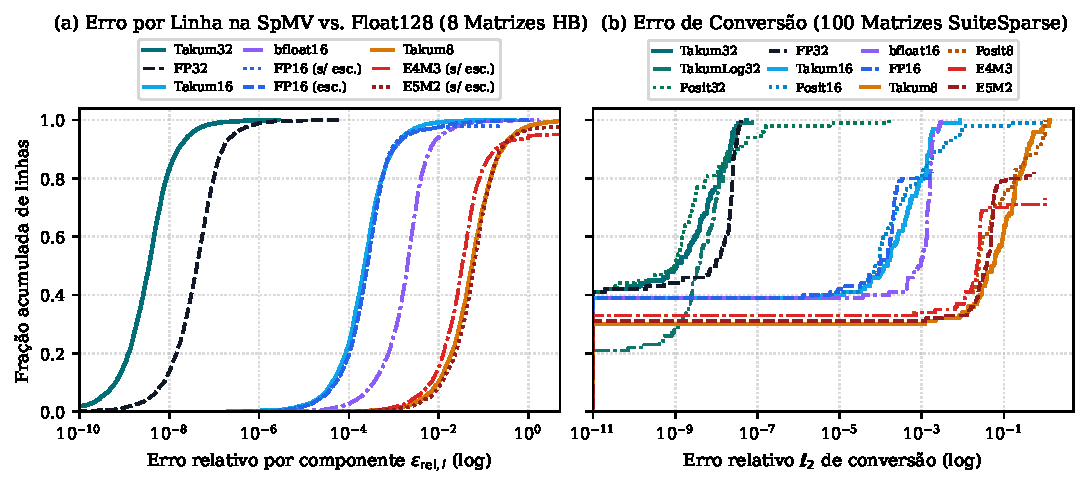
\includegraphics[width=0.77\textwidth]{figures/error-cdf-pt.pdf}
\caption{CDFs emp\'iricas frente a \texttt{Float128}: (a) erros por linha na SpMV em 8 matrizes Harwell--Boeing (74.074 avalia\c{c}\~oes; \texttt{E4M3}, \texttt{E5M2} e \texttt{FP16} n\~ao escalados terminam abaixo de 1.0 devido a \emph{overflows}), e (b) erro $\ell_2$ de convers\~ao em 100 matrizes SuiteSparse em 15 formatos, incluindo \texttt{Posit} ($es=2$) e Takum logar\'itmico.}
\label{fig:error_cdf}
\end{figure*}

\subsection{Compara\c{c}\~ao com Posits e Takum Logar\'itmico (100 Matrizes)}
\begin{table}[t]
\caption{Viabilidade de conversão em 100 matrizes SuiteSparse ($\mathrm{nnz} \le 50\,000$): Takum (Linear e Logarítmico), Posit ($es=2$) e formatos IEEE/OCP.}
\label{tab:suitesparse100}
\centering
\scriptsize
\setlength{\tabcolsep}{3.0pt}
\renewcommand{\arraystretch}{0.95}
\begin{tabular}{@{}lcccc@{}}
\toprule
Fmt. & Fin. & Mediana & P90 & Máx. \\
\midrule
OFP8 E4M3 & 73/100 & $7.17 \times 10^{-3}$ & $2.70 \times 10^{-2}$ & $1.00 \times 10^{0}$ \\
OFP8 E5M2 & 82/100 & $2.39 \times 10^{-2}$ & $5.63 \times 10^{-2}$ & $5.33 \times 10^{-1}$ \\
Posit8 & 100/100 & $2.45 \times 10^{-2}$ & $6.13 \times 10^{-1}$ & $1.07 \times 10^{0}$ \\
Takum8 (Lin.) & 100/100 & $5.35 \times 10^{-2}$ & $3.66 \times 10^{-1}$ & $1.30 \times 10^{0}$ \\
Takum8 (Log) & 100/100 & $5.42 \times 10^{-2}$ & $3.61 \times 10^{-1}$ & $3.26 \times 10^{0}$ \\
\midrule
IEEE FP16 & 82/100 & $7.58 \times 10^{-6}$ & $2.18 \times 10^{-4}$ & $1.80 \times 10^{-3}$ \\
bfloat16 & 100/100 & $8.87 \times 10^{-4}$ & $1.76 \times 10^{-3}$ & $2.96 \times 10^{-3}$ \\
Posit16 & 100/100 & $7.89 \times 10^{-5}$ & $2.79 \times 10^{-3}$ & $9.99 \times 10^{-1}$ \\
Takum16 (Lin.) & 100/100 & $1.34 \times 10^{-4}$ & $1.57 \times 10^{-3}$ & $8.49 \times 10^{-3}$ \\
Takum16 (Log) & 100/100 & $2.17 \times 10^{-4}$ & $1.31 \times 10^{-3}$ & $7.48 \times 10^{-3}$ \\
\midrule
IEEE FP32 & 100/100 & $9.64 \times 10^{-9}$ & $2.97 \times 10^{-8}$ & $4.08 \times 10^{-8}$ \\
Posit32 & 100/100 & $9.88 \times 10^{-10}$ & $3.14 \times 10^{-8}$ & $1.59 \times 10^{-4}$ \\
Takum32 (Lin.) & 100/100 & $1.06 \times 10^{-9}$ & $2.14 \times 10^{-8}$ & $5.42 \times 10^{-8}$ \\
Takum32 (Log) & 100/100 & $3.59 \times 10^{-9}$ & $1.87 \times 10^{-8}$ & $7.57 \times 10^{-8}$ \\
\bottomrule
\end{tabular}
\end{table}

A Fig.~\ref{fig:error_cdf} e a Tabela~\ref{tab:suitesparse100} ampliam o estudo para 100 matrizes SuiteSparse. Embora \texttt{Posit} obtenha mediana ligeiramente menor junto \`a unidade (\texttt{Posit16}: $7.89\times 10^{-5}$ vs.\ \texttt{Takum16}: $1.34\times 10^{-4}$), seu regime un\'ario provoca colapso severo nas caudas (\texttt{Posit16} m\'aximo de $99.9\%$ contra $0.85\%$ no \texttt{Takum16}; \texttt{Posit32} m\'aximo $1.59\times 10^{-4}$ contra $5.42\times 10^{-8}$ no \texttt{Takum32}). O Takum logar\'itmico acompanha de perto a variante linear em todas as larguras~\cite{hunhold2024takum}.

\subsection{Contagens Din\^amicas, Escritas em CSR e Modelo Anal\'itico}
\begin{table}[t]
\caption{Instru\c{c}\~oes din\^amicas, instru\c{c}\~oes \texttt{Zvtakum}, escritas em CSR e elementos ativos por n\~ao nulo, agregados nas oito matrizes Harwell--Boeing.}
\label{tab:contagens}
\centering
\scriptsize
\setlength{\tabcolsep}{3.0pt}
\renewcommand{\arraystretch}{0.95}
\begin{tabular}{@{}llcccc@{}}
\toprule
Fmt & VLEN & Insn/nnz & Zvt./nnz & CSR/nnz & Elem./nnz \\
\midrule
FP32 & 128 & 6.140 & 0.000 & 1.328 & 5.334 \\
FP32 & 256 & 4.587 & 0.000 & 1.069 & 5.334 \\
FP32 & 512 & 4.343 & 0.000 & 1.029 & 5.334 \\
\midrule
Takum32 & 128 & 5.977 & 0.497 & 1.328 & 4.501 \\
Takum32 & 256 & 4.553 & 0.368 & 1.069 & 4.501 \\
Takum32 & 512 & 4.329 & 0.347 & 1.029 & 4.501 \\
\midrule
Takum16 & 128 & 4.954 & 0.368 & 1.470 & 4.501 \\
Takum16 & 256 & 4.690 & 0.347 & 1.389 & 4.501 \\
Takum16 & 512 & 4.605 & 0.341 & 1.363 & 4.501 \\
\midrule
Takum8 & 128 & 4.510 & 0.347 & 1.389 & 4.501 \\
Takum8 & 256 & 4.431 & 0.341 & 1.363 & 4.501 \\
Takum8 & 512 & 4.392 & 0.337 & 1.350 & 4.501 \\
\bottomrule
\end{tabular}
\end{table}

\begin{table}[t]
\caption{Par\^ametros do modelo anal\'itico de contagem $N_f = r_f R + c_f S + K$, em que $R$ \'e o n\'umero de linhas e $S$ o total de faixas n\~ao vazias nas 96 execu\c{c}\~oes do simulador.}
\label{tab:modelo}
\centering
\scriptsize
\setlength{\tabcolsep}{3.0pt}
\renewcommand{\arraystretch}{0.95}
\begin{tabular}{@{}lcccrr@{}}
\toprule
Formato & $r$ & $c$ & $K$ & Sint\'eticos & Execu\c{c}\~oes exatas \\
\midrule
FP32 & 13 & 12 & 21 & 3/3 & 24/24 \\
Takum8 & 14 & 12 & 21 & 3/3 & 24/24 \\
Takum16 & 14 & 13 & 21 & 3/3 & 24/24 \\
Takum32 & 14 & 11 & 21 & 3/3 & 24/24 \\
\bottomrule
\end{tabular}
\end{table}

\begin{figure}[t]
\centering
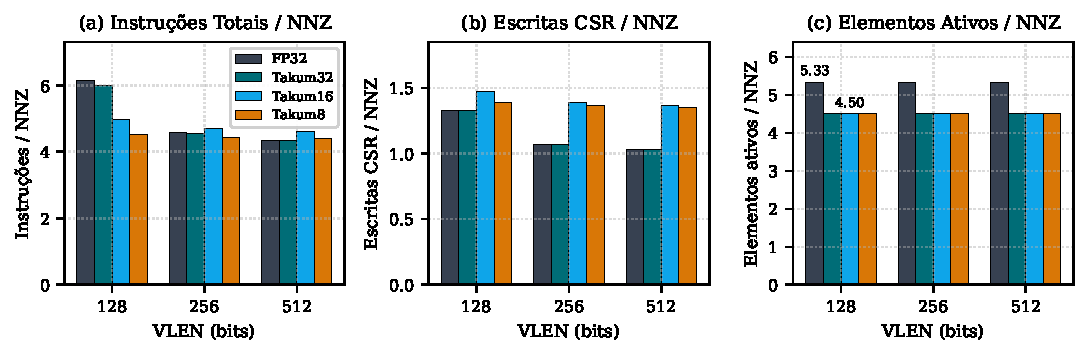
\includegraphics[width=0.78\columnwidth]{figures/insn-csr-comparison-pt.pdf}
\caption{Instru\c{c}\~oes din\^amicas, escritas em CSR e elementos vetoriais ativos por n\~ao nulo para $\mathrm{VLEN}\in\{128,256,512\}$ somados nas oito matrizes.}
\label{fig:insn_csr}
\end{figure}

Todas as \NumBitExatas\ execu\c{c}\~oes no simulador (\NumMatrizes\ matrizes $\times$ 4 formatos $\times$ 3 VLENs) conferem bit a bit com o modelo Python. As Tabelas~\ref{tab:contagens}--\ref{tab:modelo} e a Fig.~\ref{fig:insn_csr} mostram que a contagem din\^amica segue exatamente $N_f = r_f R + c_f S + K$ com res\'iduo \ModResiduoMax\ nas \ModExec\ execu\c{c}\~oes ($R$ linhas, $S$ faixas n\~ao vazias, $K=\ModKFP$). Como \texttt{vtdot.vv} funde \texttt{vfmul.vv} e \texttt{vfredusum.vs} ($c_{\text{T32}}=11 < c_{\text{FP32}}=12$) enquanto \texttt{vncvt.t.t} soma uma instru\c{c}\~ao por linha ($r_{\text{T32}}=14$ vs.\ $r_{\text{FP32}}=13$), vale $N_{\text{Takum32}} - N_{\text{FP32}} = R - S \le 0$. Assim, \texttt{Takum32} executa menos ou igual n\'umero de instru\c{c}\~oes em \InsnPares/\InsnPares\ pares (\InsnMenorTrinta\ estritamente menor, \InsnIgualTrinta\ igual), repete as escritas em CSR do \texttt{FP32} (\CsrNnzTrintaDuzentos/nnz em $\mathrm{VLEN}=256$) e reduz elementos vetoriais ativos de \ElemNnzFP\ para \ElemNnzTakum\ por n\~ao nulo ($-15.6\%$). Em 8 e 16 bits, alternar \texttt{vtype} entre \'indices de 32 bits e dados estreitos acrescenta um \texttt{vsetvli} por faixa ($+27\%\text{--}33\%$ de escritas CSR em $\mathrm{VLEN}=256$); ainda assim, em $\mathrm{VLEN}=128$, o maior empacotamento altera o total de instru\c{c}\~oes em \RelInsnDezCento\ (\texttt{Takum16}) e \RelInsnOitoCento\ (\texttt{Takum8}).

\subsection{Limita\c{c}\~oes e Escopo}
Este trabalho avalia um simulador funcional sem \emph{pipeline}, lat\^encia por ciclo, \'area ou s\'intese de pot\^encia; as m\'etricas de \texttt{FP8}/\texttt{FP16}/\texttt{bfloat16} s\~ao refer\^encias num\'ericas (n\~ao instru\c{c}\~oes \texttt{Zvfh} simuladas). O reescalamento \texttt{pow2-bound} requer duas passagens globais fora dos contadores vetoriais. A s\'intese RTL do decodificador de 12~MSBs e da unidade MAC $2\cdot\text{SEW}$ fica para trabalhos futuros.

\section{Conclus\~ao}
Projetamos, implementamos e verificamos a extens\~ao vetorial \texttt{Zvtakum} para RISC-V suportando \texttt{T8}, \texttt{T16} e \texttt{T32} via cinco instru\c{c}\~oes em \texttt{custom-0}, decodificador unificado de 12~MSBs, ULA inteira de 128 bits com RNE no espa\c{c}o de c\'odigos e elimina\c{c}\~ao de riscos em \texttt{fcsr}. Experimentos em SpMV Harwell--Boeing e 100 matrizes SuiteSparse demonstram que \texttt{Takum32} reduz o erro relativo mediano em $\RazaoKernelTrinta\times$ frente ao \texttt{FP32} sem nunca exceder sua contagem de instru\c{c}\~oes, enquanto \texttt{Takum8} e \texttt{Takum16} eliminam \emph{overflows} n\~ao finitos, superam \texttt{bfloat16} e evitam o colapso de precis\~ao dos posits nas caudas.

\bibliographystyle{IEEEtran}
\bibliography{refs}
\end{document}
